\documentclass{article}
\usepackage[a4paper, margin=1in]{geometry}
\usepackage{setspace}
% \usepackage{parskip}
\usepackage[backend=biber, sorting=none]{biblatex}
\usepackage{graphicx}
\usepackage{svg}
\usepackage{chemfig}
\usepackage{nameref}
\usepackage{hyperref}
\usepackage{tabularx}
\usepackage{multirow}
\usepackage{hhline}
\usepackage{booktabs}
\usepackage{subcaption}
\usepackage{amsmath}
\usepackage{amssymb}
\usepackage{amsfonts}
\usepackage{amsthm}
\usepackage[group-separator={,}]{siunitx}

\addbibresource{main.bib}
\graphicspath{ {./images/} }

\renewcommand{\arraystretch}{1.2}

\DeclareMathOperator*{\argmax}{argmax}
\DeclareMathOperator*{\argmin}{argmin}
\DeclareMathOperator*{\softmax}{softmax}

\begin{document}
\doublespacing

% \begin{figure}
%     \begin{subfigure}{0.49\textwidth}
%         \centering
%         \includegraphics[width=\linewidth]{}
%         \caption{}
%     \end{subfigure}
%     \caption{}
% \end{figure}

\begin{titlepage}
    \centering
    \singlespacing
    \vspace*{1cm}

    
\includegraphics[width=0.2\textwidth]{University_of_Canterbury_logo.svg.png}\\[1.5cm]

    \Huge
    \textbf{COSC681 - AI Project}\\[1.5cm]

    \LARGE
    Classifying smoking exposure with epigentic-trained machine learning\\[2cm]

    \Large
    \textbf{Lachlan Jones}\\[0.5cm]
    2025\\[1cm]

    \large
    \textbf{Supervisors:}\\
    Prof. Greg Jones (University of Otago)\\
    Prof. Richard Green (University of Canterbury)

    \vfill

    \Large
    Department of Computer Science\\
    University of Canterbury
\end{titlepage}

\pagenumbering{roman}

\begin{abstract}

\end{abstract}

\newpage
\tableofcontents

\listoffigures

\listoftables

\newpage
\pagenumbering{arabic}

\section{Introduction}
\subsection{Tobacco Related Health Issues}
The harms associated with tobacco use are well recognised. Tobacco kills up to half its users who do not quit and more than 8 million people per year, including an estimated 1.3 million non-smokers due to second hand smoke \cite{who_tobacco}. Smoking causes cancer, heart and lung disease, stroke, type 2 diabetes, and harmful reproductive effects \cite{hhs_smoking_2014}. There is a growing body of evidence suggesting a causal relationship between smoking and mental health issues \cite{taylor2019smoking}. Clearly, such negative impacts on patient health due to tobacco use are undesirable, just as they are avoidable. For these reason, tobacco usage is of great concern to health professionals. The World Health Organization asserts that surveillance is key for addressing the tobacco epidemic, as tracking tobacco usage indicates how to shape policy \cite{who_tobacco}.

\subsection{Self-Reported Smoking Status}
Current surveillance relies on self-reported smoking data. That is, a patient's smoking history is recorded by them personally recalling and reporting. It is a convenient and cost-effective way of collecting smoking statistics. There are two main types of smoking data used to measure tobacco exposure: smoking status and smoking pack-years. Smoking status is label based on the history and habits of tobacco use. Indiviudals are binned into never smokers, ex-smokers and current smokers. Smoking pack-years is a calculated score that tries to quantify tobacco use. It is calculated as the number of packs of cigarettes smoked per day multiplied by years of smoking \cite{smokingpackyears}. For example, one pack-year is one pack per day for one year, or half a pack per day for two years. Therefore, smoking pack-years quantifies both the degree of exposure and duration of exposure equally.

Self-reported smoking data has several limitations. Relying on individuals recounting information can introduce bias. Self-reported smoking data is prone to inaccuracy due to stigma, recall bias and a lack of information on second-hand exposure \cite{park2015correlation, gorber2009accuracy}. That is, the social pressure to deny partaking in stigmatised behaviours, forgetting details and information, and not being aware of sources of second-hand exposure can all influence the results of self-reported smoking data. A method of using objective evidence to determine smoking history could overcome these issues. On the other hand, the inaccuracy of self-reported smoking data can differ between population groups. For example, studies suggest that teens are more likely to provide false responses in smoking surveys \cite{park2015correlation}. Moreover, tobacco consumption differs between social groups, with smoking more prevalent in low-education and low-socio-economic groups \cite{cdc2019_smoking}.

To this end, developing diagnostic tests to collect smoking data that do not share the biases of self-reported methods are of interest for improving the monitoring of health. One such approach is the use of epigenetic biomarkers.

\subsection{Epigenetics}
Epi- is a Greek prefix meaning upon or on. Therefore, epigenetics is the study of factors on top of or upon genetics. Specifically, it is the study of how environmental factors and behaviours affect, modify and regulate your genetics and their expression. We consider one type of epigenetic modification: DNA methylation.

\begin{figure}
    \centering
    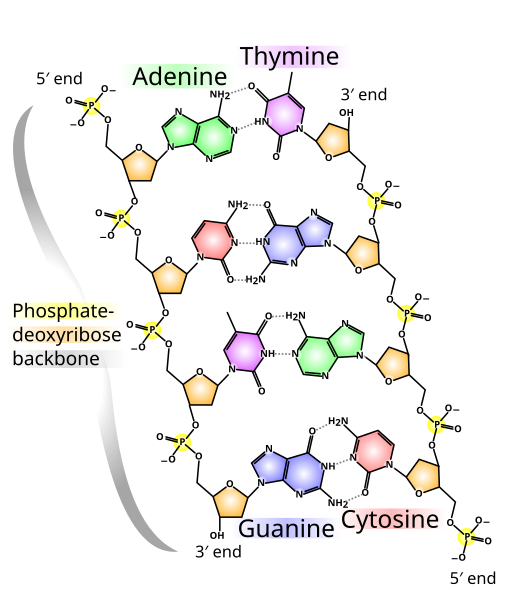
\includegraphics[width=0.5\textwidth]{512px-DNA_chemical_structure.svg.png}
    \caption*{Chemical structure of DNA \cite{ball_DNA_structure}}
\end{figure}

\subsubsection{DNA Methylation}
At a high level, DNA is a sequence of letters that provide genetic instructions. Like a human reading a book, strings of these letters are converted into information that tells cells how to function. More precisely, these letters are one of four nucleotide bases: adenine (A), cytosine (C), guanine (G) and thymine (T). To form the sequence, these bases are attached to a deoxyribose sugar and connected by a phosphate molecule, called the sugar-phosphate backbone. Of relevance is the phosphate molecule, specifically for when a cytosine is directly followed by a guanine in the sequence. A phosphate bonding a cytosine and a guanine (called a CpG site) creates a chemical structure which allows methyl groups to attach. This process is an epigenetic modification called DNA methylation (DNAm). As a biomarker, we measure methylation at a CpG site as a float between 0 and 1, measuring the percentage of methylation at that site.

While the genetic sequence of DNA is stable, methylation is not. It is a dynamic state that depends on factors such has behaviours and environmental exposure \textbf{(add citation?)}. Exposure to such factors increases methylation of CpG sites, while sufficent lack of exposure causes methylation to decrease over time \textbf{(add citation?)}. As previously mentioned, DNA methylation affects the expression of genes. Methylation at a CpG site can silence the expression of the gene that site is located in \textbf{(add citation?)}, where more methylation at a site leads to stronger silencing. Moreover, DNA methylation is not random. There is strong correlation between methylation of specific sites with specific factors \textbf{(add citation?)}. This means that DNA methylation of CpG sites can be used as a biomarker indicative of the factors that caused it, while also describing changes in cellular function. Therefore, DNA methylation is a biomarker not only useful for reporting on environmental exposures, but also predicting future health outcomes or risks. Examples of this include prediction of cardiovascular diseases \cite{cameron2023dna}, neurological diseases \cite{cells11213439}, type 2 diabetes \cite{cheng2023development}, pace of aging \cite{10.7554/eLife.73420}, and cancer \cite{luo2020circulating}. Furthermore, DNA methylation is not self-reported, and therefore overcomes the biases associated with self-reported data.

Altogether, this motivates the use of DNA methylation data to develop methods for collecting smoking history of indiviudals. Work using such data is referred to as an epigenome-wide association study (EWAS).

\begin{figure}
    \setcounter{figure}{\numexpr\value{figure}-1}
    \begin{subfigure}{0.49\textwidth}
        \centering
        \hspace*{11mm}
        \chemfig{*6(-\chembelow{N}{H}-(=O)-N=(-NH_2)-=)}
        \vspace{3mm}
        \caption{Cytosine}
    \end{subfigure}
    \begin{subfigure}{0.49\textwidth}
        \centering
        \chemfig{*6(-\chembelow{N}{H}-(=O)-N=(-NH_2)-(-H_3C)=)}
        \vspace{3mm}
        \caption{5-Methylcytosine}
    \end{subfigure}
    \caption*{Modification of Cytosine into 5-Methylcytosine caused by DNA methylation}
\end{figure}

\subsubsection{DNAm Platforms}
The human genome contains \(\sim\!28\) million CpG sites. This is often a computationally infeasible domain for a dataset, due to massive dataset sizes, processing requirements, and noise contained in the signal. Instead, most EWAS use a biologically relevant and informative subset of CpG sites. There are two commonly chosen platforms used to achieve this: Illumina 450k \cite{illumina2012methylation450} and Illumina EPIC \cite{illumina2015methylationepic}. 450k was the first array developed by Illumina, consisting of \num{485577} CpG sites chosen for their quality and usefulness. The EPIC array was developed as a successor, increasing to \num{865859} CpG sites. However, only around \(>90\%\) of the sites were retained from 450k. This is something that needs to be considered when developing scores or screening tests from an EWAS if compatability with multiple datasets or cohorts is of concern (see \ref{sec:pre-processing}).

Additionally, these arrays are compatible with DNA from multiple different cell types. Some examples include whole blood, purified cells and fresh-frozen tissue \cite{bhat2022data}. Moreover, the methylation signal can differ across different cell types \cite{huang2016epigenome}, which means selection of cell type can be an import factor when designing an EWAS. Typically, whole blood is used, specifically white blood cells, as red blood cells in humans do not carry a copy of the DNA.

% \vspace{1cm}
% \begin{itemize}
%     \item At a high level, DNA is a sequence of letters that provide genetic instructions
%     \item nucleotide bases (A, T, C, G) connected with a phosphate sugar backbone
%     \item Cs next to Gs create a chemical structure that allows methyl groups to attach: CpG site, = epigenetic modification
%     \item description of what the word epigenetics, "upon" genetics
%     \item While genetic sequence is stable, methylation is a dynamic state which depends on factors, enviroment etc.
%     \item The state of methylation can change/effect the expression of genes, where methylation = silencing.
%     \item Methylation isn't random, with strong correlation between methylation of specific CpG sites with specific factors
%     \item This means methylation status can be used as a biomarker for indicating and reporting on environmental exposures and report on health outcomes
%     \item Status of methylation sites can determine health outcomes, including cancer risk, CVD, diabetes, etc.
% \end{itemize}

% \subsubsection{DNAm Platforms}

% \begin{itemize}
%     \item Two types of DNAm platform, illumina 450k and illumina EPIC
%     \item \(\sim\)28 million CpG sites in the human genome, platforms choose specific sites to ranked
%     \item Cell type of sample matters, different cells with have different methylation. Typically whole blood is used, good general methylation signal.
% \end{itemize}

\subsection{Machine Learning in Epigenetics}
Broadly, machine learning algorithms are split into one of two tasks: regression or classification. The most significant distinction between these two tasks is the choice of supervised learning labels. Regression algorithms are trained against continuous, numeric scores, while classification algorithms are trained against discrete class labels. The choice of label in turn determines the output produced by the algorithm.
Machine learning has already seen use in many areas of clinical epigenetics. We begin with a review of some developed methods, addressing both classification and regression tasks.

\subsubsection{Applications} \label{sec:ml-examples}
\begin{enumerate}
    \item Malta et al. \cite{malta2018machine} proposed a method for assessing oncogenic dedifferentiation (cells becoming cancerous). This approach seeks to model a "stemness index" which indicates how similar a cell is to stem cell - a trait found in cancerous cells. Of relevance is the developed epigenetic approach using one-class logistic regression. The training features consisted of 219 hypermethylated CpG sites associated with stem cells. Training data only consisted of a single, positive, class: stem cells. The resulting model can then be fed non-stem cells to compare how similar they are to stem cells, i.e. cancerous cells.

    \item Adorj\'an et al. \cite{adorjan2002tumour} proposed a method for using DNA methylation to classify cancer tissues. CpG sites were ranked using a two sample t-test, and then fed into a support vector machine. Models were evaluated using the average of 50 runs of 8-fold cross-validation. The top two CpG sites could classify leukaemia from healthy cells with 84\% accuracy, while the top 60 sites achieve 94\% accuracy.

    \item Dogan et al. \cite{dogan2018integrated} proposed a method for integrated genetic and epigenetic classification of coronary heart disease. The training dataset consisted of 1,545 indiviudals. An approach combining undersampling and ensemble learning \cite{liu2008exploratory} was used to address class imbalance, creating 8 training sub-datasets. Point biserial correlation and Pearson correlation were used for feature selection, resulting in 107,799 CpG sites for training. These features were ranked using ROC AUC. Random Forest classifiers were then trained on the 8 training sub-datasets, with majority voting used for ensembling. Hyperparameters were tuned using 10-fold cross-validation. The final model used 4 CpG cites, two genetic variables, age and sex. This achieved an accuracy, sensitivity and specificity of 78\%, 0.75 and 0.80, respectively.
\end{enumerate}

\subsection{Smoking Algorithms}
In the context of smoking, the two most significant machine learning epigenetic scores use Elastic Net regression.

\subsubsection{Elastic Net Regression}
Elastic Net \cite{zou2005regularization} is a regularised form of linear regression that includes two additional penalty terms.
Given \(n\) examples, \(p\) features with inputs \(x \in \mathbb{R}^{n \times (p + 1)}\) and corresponding ground-truth \(y \in \mathbb{R}^n\), we find coefficients \(\beta \in \mathbb{R}^{p + 1}\) that produces an output:
\[\hat{y} = x \beta \in \mathbb{R}^{p + 1}\]
and minimises the function:
\[\mathcal{L}(y, \hat{y}, \beta) = ||y - \hat{y}||_2^2 + \alpha\lambda||\beta||_1 + \alpha\frac{1 - \lambda}{2}||\beta||_2^2\]
where:
\[||\beta||_1 = \sum_{i=1}^{p} |\beta_i|\]
and:
\[||\beta||_2 = \sqrt{\sum_{i=1}^{p} \beta_i^2}\]

We can see this is simply mean-squared error, with the \(L_1\)-norm and \(L_2\)-norm included as penalisation terms on \(\beta\). The two hyperparameters \(\alpha\) and \(\lambda\) control the strength of regularisation and ratio between \(L_1\)-norm and \(L_2\)-norms, respectively. Elastic Net is a combination of two other modifications to linear regression: lasso \cite{tibshirani1996regression} and ridge \cite{hoerl1970ridge} regression. The two mathematical regularisation terms have interpretable effects on the convergence of \(\beta\). Gradient updates for \(||\beta||_1\) are uniform for all non-zero values of \(\beta_i\), which typically results in most \(\beta_i\) set to zero, with some having large values. This is referred to as a sparse solution. Gradient updates for \(||\beta||_2^2\) are large for large \(\beta_i\), and small for small \(\beta_i\), which typically results in all \(\beta_i\) having similar values. This is referred to as shrinkage. Together, this results in Elastic Net models promoting the grouping effect, where strongly related features are all included or excluded together. This grouping effect is particularly useful when \(p > n\), as it provides better feature selection than lasso \cite{zou2005regularization}. Because of this, Elastic Net sees wide use in epigenetics, with biological age clocks being one area of particular use \cite{teschendorff2025epigenetic}.

\subsubsection{DNAmPACKYRS} \label{sec:dnampackyrs}
Lu et al. \cite{lu2019dna} proposed DNAmPACKYRS as a DNA methylation based score for calculating smoking pack-years. This score was originally developed as surrogate biomarker for use in the DNAm GrimAge and DNAm GrimAge v2 epigenetic clocks \cite{lu2019dna,lu2022dna}. DNAm GrimAge is a regression model for estimating mortality risk. The DNAm GrimAge score is calculated using covariates sex, age, 7 surrogate biomarkers of plasma proteins, and of relevance, the surrogate biomarker for smoking pack-years: DNAmPACKYRS. Elastic Net regression was used to train both DNAm GrimAge and the surrogate biomarkers of plasma proteins and pack-years. Training data consisted of 1731 individuals from the Framingham Heart Study dataset \cite{doi:10.2105/AJPH.41.3.279}. Indiviudals from this dataset had a mean age of 66 years. 54\% of individuals were female, leaving 45\% as male. The intersection of sites available on Illumina 450k and Illumina EPIC were chosen as the available CpG sites for training. This was to ensure compatability and future-proofing with new datasets. A total of \num{450161} CpG sites were available. 10-fold cross-validation was used for hyperparameter tuning the regularisation strength of the Elastic Net model. This resulted in the DNAmPACKYRS score which used 172 CpG sites.

As surrogate biomarker for lifespan, DNAmPACKYRS performs better than self-reported pack-years. Firstly, DNAmPACKYRS can be used to predict lifespan in never-smokers \cite{lu2019dna}, whereas self-reported pack-years cannot (all self-reported values would be 0). Additionally, DNAmPACKYRS is a more significant predictor of lifespan than self-reported pack-years. Across 4 out of 5 datasets DNAmPACKYRS had a smaller Cox regression p-values when compared to self-reported pack-years \cite{lu2019dna}.
% \(8.10\mathrm{e}{-23}\) vs \(1.12\mathrm{e}{-11}\), \(8.51\mathrm{e}{-5}\) vs \(2.13\mathrm{e}{-3}\), \(7.17\mathrm{e}{-12}\) vs \(7.03\mathrm{e}{-12}\), \(2.1\mathrm{e}{-19}\) vs \(6.4\mathrm{e}{-19}\), and \(5.33\mathrm{e}{-4}\) vs \(1.78\mathrm{e}{-1}\), respectively. 

There are some limitations with the DNAmPACKYRS score. Since DNAmPACKYRS is only evaluated as a surrogate biomarker in the GrimAge paper, there is no reporting on its performance of predicting smoking status. However, this can be done independently (see \ref{sec:val-cohort}). When performed, we can see that while DNAmPACKYRS achieves good predictive performance seperating never smokers from current smokers (ROC AUC = 0.991) and ex-smokers from current smokers (ROC AUC = 0.915), the score is not optimised for seperating never smokers from ex-smokers (ROC AUC = 0.798). Additionally, the choice of self-reported pack-years as a regression label introduces a source of inaccuracy, discussed below (see \ref{sec:mcigarette}: \nameref{sec:mcigarette}).

% Notes for DNAmPACKYRS/mCigarette:
% \begin{itemize}
%     \item dataset/cohort/demographic
%     \item algorithms
%     \item result/stat it produces
%     \item limitations
% \end{itemize}

\subsubsection{mCigarette} \label{sec:mcigarette}
Chybowska et al. \cite{chybowska2025blood} proposed mCigarette as a DNA methylation based score for calculating pack-years. This score was part of the very recent (2025) study comparing brain- and blood-based DNA methylation associated with smoking. This worked aimed to overcome the limitations of self-reported smoking data, as well as the modest performance of seperating never smokers from ex-smokers of previous studies. Several techniques were employed, including high resolution approaches involving \(\sim \! 20\) million CpG sites. The most relevant method is the developed smoking biomarker: mCigarette. Similar to DNAmPACKYRS, this is a methylation based score for smoking pack-years trained with Elastic Net Regression. Training data consisted of \num{17865} indiviudals from the Generation Scotland dataset \cite{smith2006generation}, which was developed on the Illumina EPIC array. Individuals from this dataset had a mean age of 47.6 years. 59.1\% of the individuals were female. CpG sites were filtered based on statisticcal association with tobacco use at a false discovery rate (FDR) \(< 0.05\), resulting in \num{18760} CpG sites per indiviudal. This filtering was ran in a dataset seperate to the training dataset, using the Illumina 450k array. Note that this limits training features those CpG sites found on both the 450k and EPIC arrays. Elastic Net regression was then used to train the mCigarette score. Hyperparameters were tuned using 10-fold cross-valdiation, which set \(\lambda = 0.012577\) and resulted in a model using \num{1255} CpG sites.

As a result, mCigarette achieves incremental performance on previous scores. In an independent validation cohort, mCigarette achieves ROC AUCs of 0.98, 0.90 and 0.85 for current vs never, current vs ex- and never vs ex- smokers, respectively.

% Two ex-smokers (both 70 years of age) with the same pack year value but very different smoking-related chronic disease risk.  Person A gave up smoking 1year ago but had smoked half a pack a day for the last 40 years (20 pack years), Person B smoked 2 packs a day from 15-25 years age (20 pack years) but hasn’t smoked in 45 years.  Chronic disease (eg. Lung cancer and heart disease) risk is much higher in person A than B.  Moreover, we would expect very different smoking related DNA methylation values between the two people.

There are limitations associated with the mCigarette score. The choice of smoking pack-years may be inaccurate as a training marker, due to the potential to label two individuals with siginificantly different smoking exposure as the same. As an example, consider two ex-smokers both of 70 years of age. Individual A gave up smoking 1 year ago, but smoked half a pack of cigarettes per day for 40 years prior, which equates to 20 pack-years. Individual B smoked 2 packs of cigarettes per day from ages 15 to 25 but has quit since, which also equates to 20 pack-years. Both individuals have the same smoking pack-years score, but different lengths of cessation (1 year vs 45 years). This is problematic, as risk of chronic disease (e.g. lung cancer and cardiovascular disease) would be expected to be much higher in individual A than individual B, as duration of smoking carries greater risk than intensity of smoking \cite{potter2024pack}. Moreover, we would expect different smoking-related methylation signals for the two individuals. Thus, individuals with less intense but longer duration of smoking exposure may have underestimated smoking exposure by such a model. Therefore, smoking pack-years is an inaccurate choice of training label, as it does not capture the importance of length of smoking cessation. Note that this limitation is also associated with the DNAmPACKYRS score.

% \begin{itemize}
%     \item[\checkmark] (?) seeking to address not being able to differentiate never smokers and ex-smokers
%     \item[\checkmark] 17865 indiviudals
%     \item[\checkmark] filtered CpG sites to FDR \(< 0.05\) \((n = 18760)\)
%     \item[\checkmark] elastic net regression
%     \item[\checkmark] 10-fold cross-validation, \(\lambda = 0.012577\)
%     \item[\checkmark] 1255 CpG sites used in model
%     \item[\checkmark] in validation cohort, AUCs of Current vs Never: 0.98, Current vs Former: 0.90, Former vs Never: 0.85
%     \item limitation 2: choice of ground truth (sr pack-years) is potentially confusing for the model
% \end{itemize}

\subsection{Aim of This Work}

As mentioned above, there are limitations associated with using smoking pack-years as a training label, largely due to not acounting for length of smoking cessation. This could be addressed by correcting smoking pack-year values for length of smoking cessation, however, both self-reported smoking pack-years and self-reported length of smoking cessation have concerns for bias associated with self-reported data. Instead, self-reported smoking status (current, ex- or never smoker) is deemed to be a more reliable and complete measure of smoking exposure.

Therefore, we reframe modeling smoking history as a classification task rather than a regression task (\ref{sec:algorithm}). This changes aims to overcome the described limitations of using smoking pack-years as a training label to achieve better class seperation between never smokers and ex-smokers. We first use individuals' self-reported smoking status to identify differentially methylated CpG sites as a feature selection step in our training dataset (\ref{sec:feature-selection}). These sites are then used to train a multi-class logistic regression model (\ref{sec:training}), which is validated in a hold-out test dataset (\ref{sec:cohort1-performance}) and independent validation cohort (\ref{sec:cohort2-performance}). Additionally, the independent validation cohort is used to compare our model with the two existing gold standard models: DNAmPACKYRS and mCigarette (\ref{sec:model-comparison}).

\section{Method}

\subsection{Algorithm} \label{sec:algorithm}
We begin by transforming Elastic Net from a regression problem into a classification problem. In the binary classification case, this is a straightforward replacement of the mean-square error term in the loss function with a binary-cross entropy error term, alongside transforming the linear prediction into a probability via the sigmoid function. However, in the multiclass classification case the modification also affects the regularisation terms.

Given \(n\) examples, \(p\) features, \(K\) classes with inputs \(x \in \mathbb{R}^{n \times (p + 1)}\) and corresponding ground-truth (as one-hot encoded vectors) \(y \in \mathbb{R}^{n \times K}\), we find coefficients \(\beta \in \mathbb{R}^{K \times (p + 1)}\) that produces logits:
\[z = x \beta^\mathsf{T} \in \mathbb{R}^{n \times K}\]
We transform this into probabilities with the softmax function:
\[\softmax(t_1,... , t_k) =
    \begin{bmatrix}
        \frac{\exp(t_1)}{\sum_{j=1}^{K} \exp(t_j)} \\
        \vdots                                     \\
        \frac{\exp(t_k)}{\sum_{j=1}^{K} \exp(t_j)}
    \end{bmatrix}
\]
The loss function then becomes:
\[\mathcal{L}(y, z, \beta) = -\frac{1}{n}\sum_{i=1}^{n} y_i \cdot \log(\softmax(z_i)) + \alpha\sum_{k=1}^{K}(\lambda||\beta_k||_1 + (1 - \lambda)||\beta_k||_2^2)\]
where the \(L_1\)-norm and \(L_2\)-norm are as before.

Colloquially, this model can be thought of as training \(K\) indiviudal logistic regression sub-classifiers, where each sub-classifier is tasked only with predicting one of the \(K\) classes. The softmax function ensures that for each example, the \(K\) predicted probabilities will all add to 1. Regularisation terms work as before, but are now per-sub-classifier.

Implementation of multi-class Elastic Net logistic regression is provided by scikit-learn \cite{scikit-learn}, via the \verb|linear_model.LogisticRegression| class.

\subsection{Datasets}
This work uses two datasets, a discovery cohort and a valdiation cohort. \textbf{(Note for editor: I want to make a comment at some point for the computer scientists reading this on why we have two cohorts [instead of combining them like we would in CS]. Should I do it here, or in the discussion/results?)}

Put it in discussion, but reference that section here. 

\subsubsection{Cohort 1: Discovery}
Cohort 1 contains DNA methylation data for 943 individuals. Across these individuals, 100\% are male, and there is a mean age of 72 years. Data was collected using the Illumina 450k array, which measured the methylation of \num{449521} CpG sites using the white blood cells found in whole blood samples. To ensure model compatability with independent datasets, available CpG sites were restricted to those found on both Illumina 450k and EPIC. This reduced available CpG sites by \(\sim\!90\%\). Note that this practice is consistent with previous work \textbf{(Note for editor: should I referrence the section I've written or the original paper here?)} (see \ref{sec:dnampackyrs}/DNAmPACKYRS \cite{lu2019dna} \ref{sec:mcigarette}/mCigarette \cite{chybowska2025blood}). Alongside epigenetic data, age, sex, self-reported pack-years and self-reported smoking-status were also recorded. Of the 943 individuals, 235 are never smokers, 599 are ex-smokers and 109 are current smokers. 90\% of this cohort was used as the model's training dataset, while the remaining 10\% was reserved as a test set to evaluate model performance. This was done in a stratified manner, which preserved the class balance from the original cohort.

% \begin{itemize}
%     \item[\checkmark] Illumina 450k
%     \item[\checkmark] all males
%     \item[\checkmark] mean age 72
%     \item[\checkmark] 235 never smokers, 599 ex smokers, 109 current smokers
%     \item 90/10 train/test split
%           \begin{itemize}
%               \item 211 never smokers, 539 ex smokers, 98 current smokers in training split
%               \item 24 never smokers, 60 ex smokers, 11 current smokers in test split
%           \end{itemize}
%     \item[\checkmark] \num{449521} CpG sites
%     \item[\checkmark] white blood cells from whole blood
% \end{itemize}

\subsubsection{Cohort 2: Validation}
Cohort 2 contains DNA methylation data for 984 individuals. Across these individuals 67\% are male, and there is a mean age of 68 years. Data was collected using the Illumina EPIC array, which measured \num{865,859} CpG sites using the white blood cells found in whole blood samples. Because the model was trained on a dataset using the 450k array, the available sites in this evaluation dataset were restricted to those found on both Illumina 450k and EPIC. This reduced available CpG sites by \(\sim\!50\%\). Alongside epigenetic data, age, sex, self-reported pack-years and self-reported smoking-status were also recorded. Of the 984 individuals, 403 are never smokers, 476 are ex-smokers and 105 are current smokers. In addition to independently validating the trained model's performance, this dataset is used to compare the trained model to the externally-derived, existing gold standard models. 

% \begin{itemize}
%     \item Illumina EPIC
%     \item 67\% of individuals were male (n=658) (female n=326)
%     \item mean age 68
%     \item 403 never smokers, 476 ex smokers, 105 current smokers
%     \item \num{449521} CpG sites (intersection with 450k)
%     \item white blood cells from whole blood
% \end{itemize}

% \begin{table}
%     \caption{Datasets Comparisons}
%     \begin{tabularx}{\textwidth}{|X|l|r|r|r|}
%         \hline
%         \multicolumn{2}{|c|}{\textbf{Metric}}    & \textbf{Cohort 1 - Train} & \textbf{Cohort 1 - Test} & \textbf{Cohort 2}                     \\
%         \hline
%         \multicolumn{5}{|c|}{\textbf{Class Balance}}                                                                                            \\
%         \hline
%         \multicolumn{2}{|l|}{Num. Individuals}   & \num{848}                 & \num{95}                 & \num{984}                             \\
%         \hline
%         \multirow{2}{*}{Never Smokers}           & Count                     & \num{211}                & \num{24}          & \num{403}         \\
%         \cline{2-5}
%                                                  & Percent                   & \SI{25}{\percent}        & \SI{25}{\percent} & \SI{41}{\percent} \\
%         \hline
%         \multirow{2}{*}{Ex-Smokers}              & Count                     & \num{539}                & \num{60}          & \num{476}         \\
%         \cline{2-5}
%                                                  & Percent                   & \SI{63.5}{\percent}      & \SI{63}{\percent} & \SI{48}{\percent} \\
%         \hline
%         \multirow{2}{*}{Current Smokers}         & Count                     & \num{98}                 & \num{11}          & \num{105}         \\
%         \cline{2-5}
%                                                  & Percent                   & \SI{11.5}{\percent}      & \SI{12}{\percent} & \SI{11}{\percent} \\
%         \hline
%         \multicolumn{5}{|c|}{\textbf{Cohort Distribution}}                                                                                      \\
%         \hline
%         \multicolumn{2}{|l|}{Percent. Male}      & \SI{100}{\percent}        & \SI{100}{\percent}       & \SI{67}{\percent}                     \\
%         \hline
%         \multicolumn{2}{|l|}{Mean Age}           & \num{72}                  & \num{71.5}               & \num{68}                              \\
%         \hline
%         \multicolumn{5}{|c|}{\textbf{Num. CpG Sites}}                                                                                           \\
%         \hline
%         \multicolumn{2}{|l|}{Raw Illumina Array} & \num{485577}              & \num{485577}             & \num{865859}                          \\
%         \hline
%         \multicolumn{2}{|l|}{Post-intersection}  & \num{449521}              & \num{449521}             & \num{449521}                          \\
%         \hline
%         \multicolumn{2}{|l|}{Percent. Retained}  & \SI{93}{\percent}         & \SI{93}{\percent}        & \SI{52}{\percent}                     \\
%         \hline
%     \end{tabularx}
% \end{table}

\begin{table}
    \caption{Datasets Comparisons}
    \begin{tabularx}{\textwidth}{X l r r r}
        \toprule
        \multicolumn{2}{c}{\textbf{Metric}}    & \textbf{Cohort 1 - Train} & \textbf{Cohort 1 - Test} & \textbf{Cohort 2}                     \\
        \addlinespace
        \multicolumn{5}{c}{\textbf{Class Balance}}                                                                                            \\
        \midrule
        \multicolumn{2}{l}{Num. Individuals}   & \num{848}                 & \num{95}                 & \num{984}                             \\
        \cmidrule(lr){1-2}
        \multirow{2}{*}{Never Smokers}         & Count                     & \num{211}                & \num{24}          & \num{403}         \\
                                               & Percent                   & \SI{25}{\percent}        & \SI{25}{\percent} & \SI{41}{\percent} \\
        \cmidrule(lr){1-2} % \cmidrule(lr){3-5}
        \multirow{2}{*}{Ex-Smokers}            & Count                     & \num{539}                & \num{60}          & \num{476}         \\
                                               & Percent                   & \SI{63.5}{\percent}      & \SI{63}{\percent} & \SI{48}{\percent} \\
        \cmidrule(lr){1-2} % \cmidrule(lr){3-5}
        \multirow{2}{*}{Current Smokers}       & Count                     & \num{98}                 & \num{11}          & \num{105}         \\
                                               & Percent                   & \SI{11.5}{\percent}      & \SI{12}{\percent} & \SI{11}{\percent} \\
        \addlinespace
        \multicolumn{5}{c}{\textbf{Cohort Distribution}}                                                                                      \\
        \midrule
        \multicolumn{2}{l}{Percentage Male}      & \SI{100}{\percent}        & \SI{100}{\percent}       & \SI{67}{\percent}                     \\
        \multicolumn{2}{l}{Mean Age}           & \num{72}                  & \num{71.5}               & \num{68}                              \\
        \addlinespace
        \multicolumn{5}{c}{\textbf{Num. CpG Sites}}                                                                                           \\
        \midrule
        \multicolumn{2}{l}{Raw Illumina Array} & \num{485577}              & \num{485577}             & \num{865859}                          \\
        \multicolumn{2}{l}{Post-intersection}  & \num{449521}              & \num{449521}             & \num{449521}                          \\
        \multicolumn{2}{l}{Percentage Retained}  & \SI{93}{\percent}         & \SI{93}{\percent}        & \SI{52}{\percent}                     \\
        \bottomrule
    \end{tabularx}
\end{table}

\subsection{Hardware and Software}
\begin{itemize}
    \item Apple M2
    \item Memory (and limitations)
          \begin{itemize}
              \item relevant to aspects of training and preprocessing (see Kruskal-Wallis)
          \end{itemize}
    \item Python version and package versions (sklearn, numpy, scipy)
    \item bench mark training times and memory use
\end{itemize}

\subsection{Pre-Processing} \label{sec:pre-processing}
\begin{itemize}
    \item Limiting both datasets to the intersection of 450k and EPIC
    \item Formatting to csv/transposing for ML
\end{itemize}

\subsubsection{Feature Selection} \label{sec:feature-selection}
\begin{itemize}
    \item Kruskal-Wallis feature selection \cite{Kruskal1952UseOR}
          \begin{itemize}
              \item "differentially methylated"
          \end{itemize}
\end{itemize}

\subsection{Training} \label{sec:training}
\begin{itemize}
    \item Cross Validation
          \begin{itemize}
              \item 10 folds
              \item stratified folds (same proportion of classes in each fold)
              \item coarse to fine approach
              \item f1-macro scoring (instead of neg log loss)
          \end{itemize}
    \item choice of optimiser/solver
    \item choice of loss function
    \item class weight balancing for gradient updates

\end{itemize}

\section{Results} \label{sec:results}

\subsection{Model Performance} \label{sec:cohort1-performance}

\begin{itemize}
    \item Confusion Matrices:
          \begin{itemize}
              \item Good accuracy/tpr across all three classes
          \end{itemize}
    \item
\end{itemize}

\begin{figure}
    \begin{subfigure}{0.49\textwidth}
        \centering
        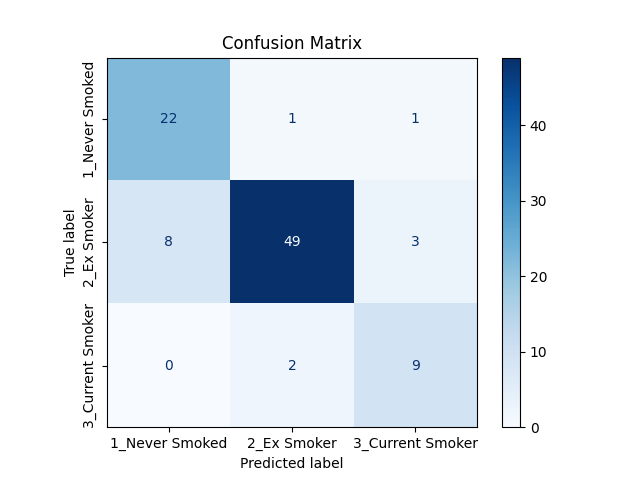
\includegraphics[width=\linewidth]{cohort1_cm.png}
        \caption{CM}
    \end{subfigure}
    \hfill
    \begin{subfigure}{0.49\textwidth}
        \centering
        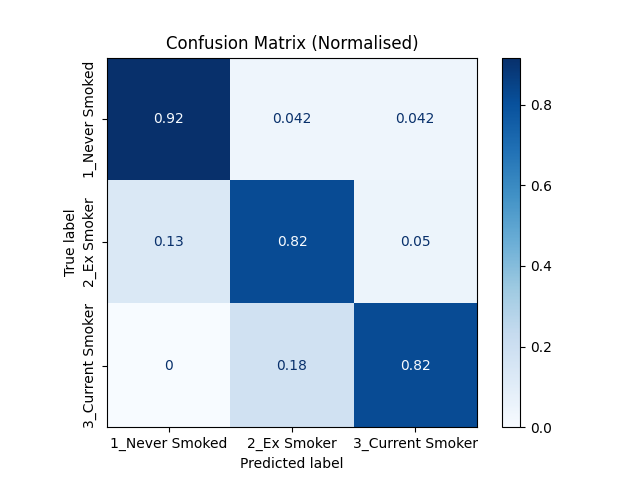
\includegraphics[width=\linewidth]{cohort1_cm_n.png}
        \caption{CM Normalised}
    \end{subfigure}
    \caption{Confusion Matrices (Cohort 1)}
\end{figure}

\begin{figure}
    \begin{subfigure}{0.48\textwidth}
        \centering
        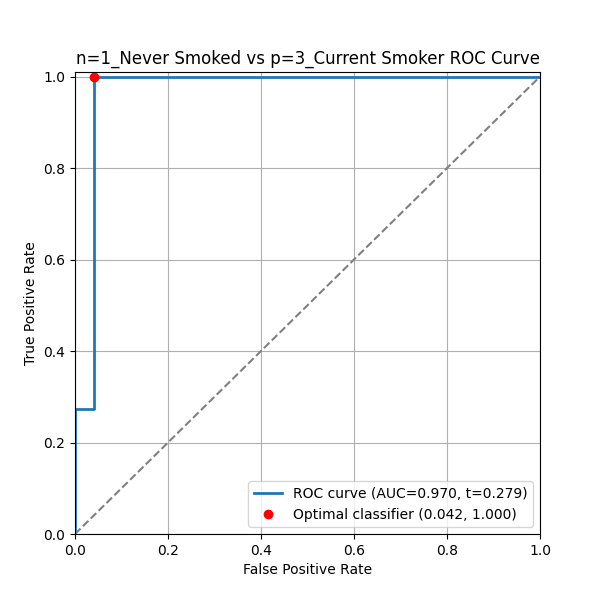
\includegraphics[width=\linewidth]{cohort1_1v3_roc.png}
        \caption{Seperation of never vs current smokers by current smoker sub-classifier}
    \end{subfigure}
    \hfill
    \begin{subfigure}{0.48\textwidth}
        \centering
        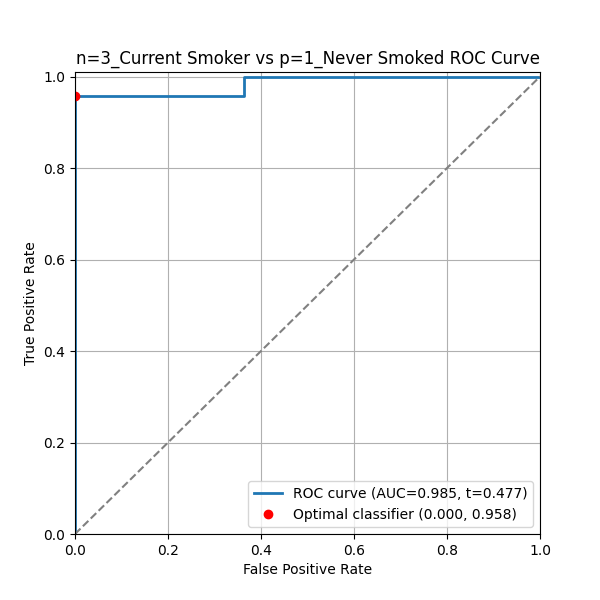
\includegraphics[width=\linewidth]{cohort1_3v1_roc.png}
        \caption{Seperation of never vs current smokers by never smoker sub-classifier}
    \end{subfigure}
    \caption{Never smoker vs current smoker sub-classifiers performance (Cohort 1)}
\end{figure}

\begin{figure}
    \begin{subfigure}{0.48\textwidth}
        \centering
        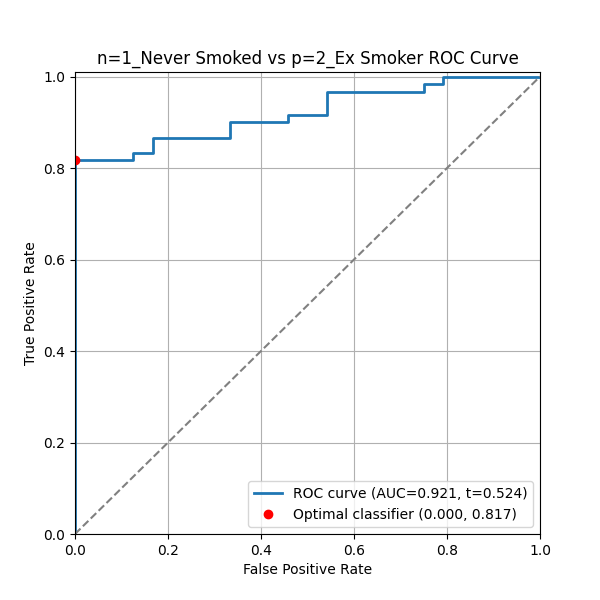
\includegraphics[width=\linewidth]{cohort1_1v2_roc.png}
        \caption{Seperation of never vs ex-smokers by ex-smoker sub-classifier}
    \end{subfigure}
    \hfill
    \begin{subfigure}{0.48\textwidth}
        \centering
        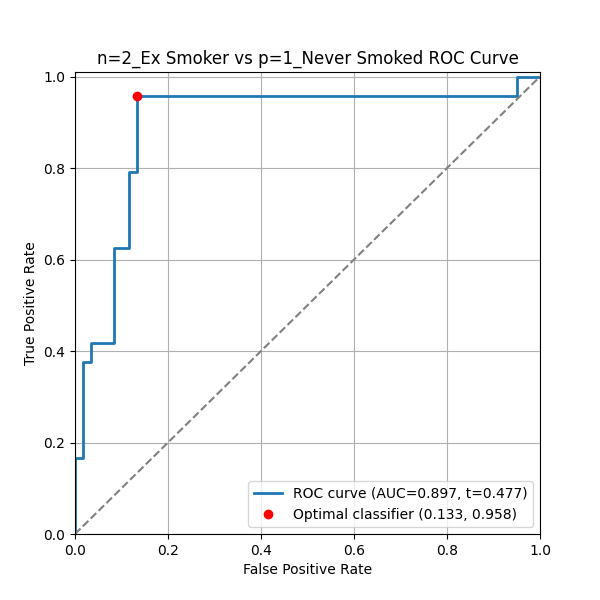
\includegraphics[width=\linewidth]{cohort1_2v1_roc.png}
        \caption{Seperation of never vs ex-smokers by never smoker sub-classifier}
    \end{subfigure}
    \caption{Never smoker vs ex-smoker sub-classifiers performance (Cohort 1)}
\end{figure}

\begin{figure}
    \begin{subfigure}{0.48\textwidth}
        \centering
        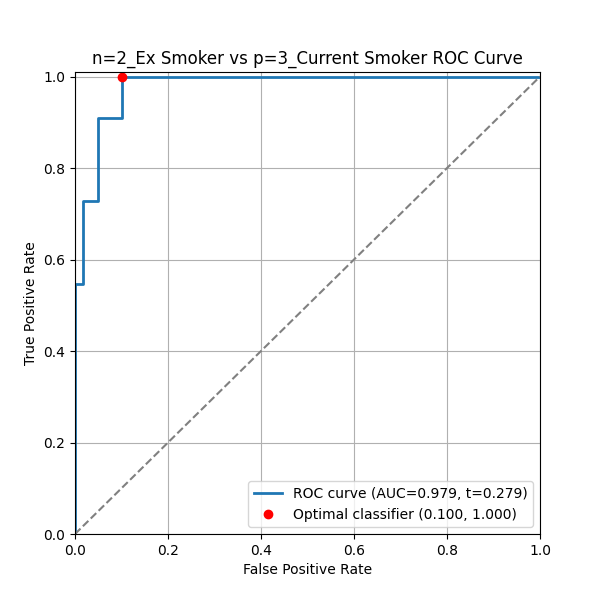
\includegraphics[width=\linewidth]{cohort1_2v3_roc.png}
        \caption{Seperation of ex vs current smokers by current smoker sub-classifier}
    \end{subfigure}
    \hfill
    \begin{subfigure}{0.48\textwidth}
        \centering
        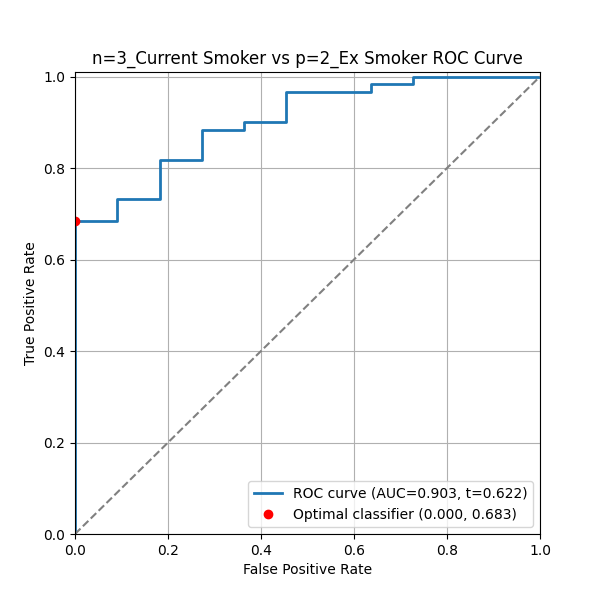
\includegraphics[width=\linewidth]{cohort1_3v2_roc.png}
        \caption{Seperation of ex vs current smokers by ex-smoker sub-classifier}
    \end{subfigure}
    \caption{Ex-smoker vs current smoker sub-classifiers performance (Cohort 1)}
\end{figure}

\begin{figure}
    \centering
    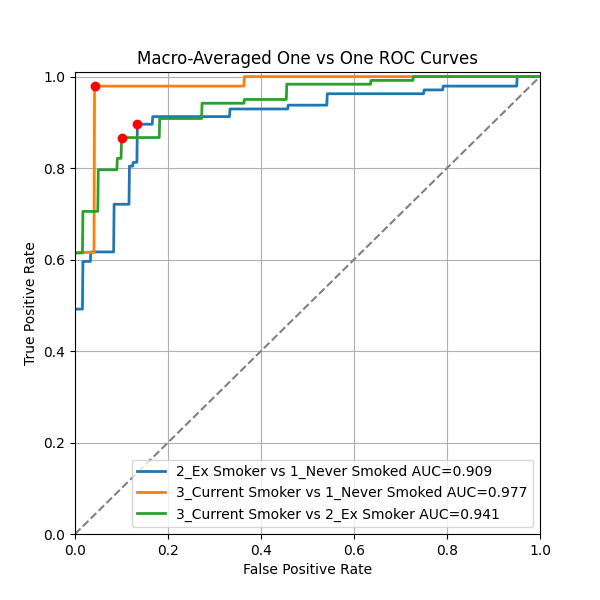
\includegraphics[width=\linewidth]{cohort1_macro_ovo_roc.png}
    \caption{Class seperation of classifier (Cohort 1)}
\end{figure}

\begin{figure}
    \centering
    \begin{subfigure}{0.48\textwidth}
        \centering
        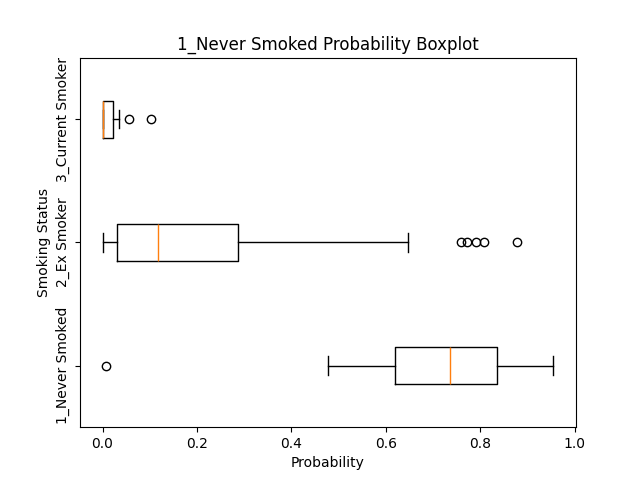
\includegraphics[width=\linewidth]{cohort1_1_boxplot.png}
        \caption{Never smoker sub-classifier probabilities across all three classes}
    \end{subfigure}
    \hfill
    \begin{subfigure}{0.48\textwidth}
        \centering
        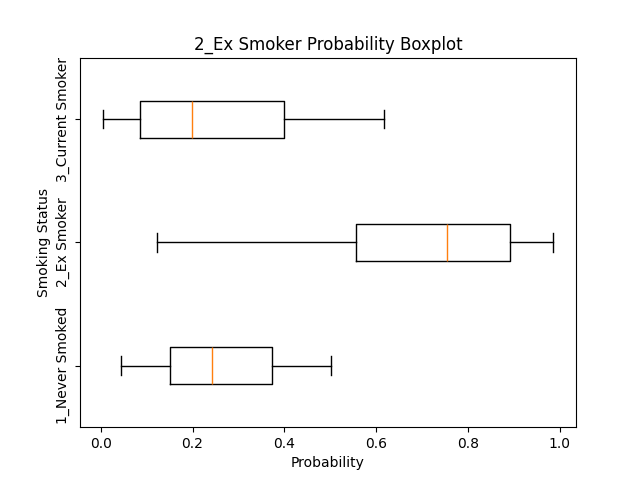
\includegraphics[width=\linewidth]{cohort1_2_boxplot.png}
        \caption{Ex-smoker sub-classifier probabilities across all three classes}
    \end{subfigure}
    \par\vspace{0.5em}
    \begin{subfigure}{0.48\textwidth}
        \centering
        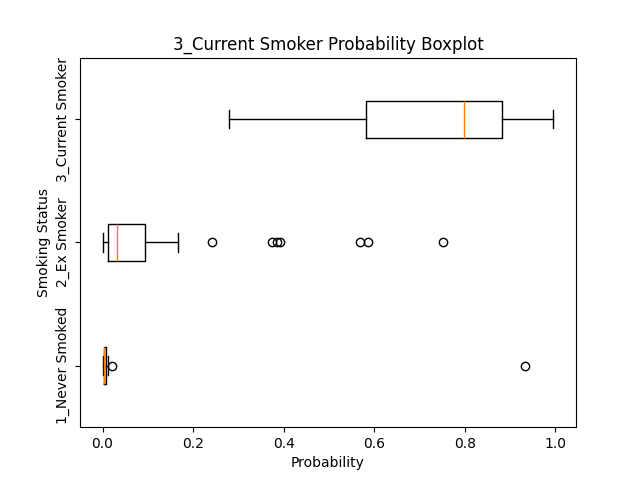
\includegraphics[width=\linewidth]{cohort1_3_boxplot.png}
        \caption{Current smoker sub-classifier probabilities across all three classes}
    \end{subfigure}
    \caption{Boxplots of probability distributions (Cohort 1)}
\end{figure}

\subsection{External Validation Cohort} \label{sec:val-cohort}
\subsubsection{Model Performance} \label{sec:cohort2-performance}
\begin{figure}
    \begin{subfigure}{0.49\textwidth}
        \centering
        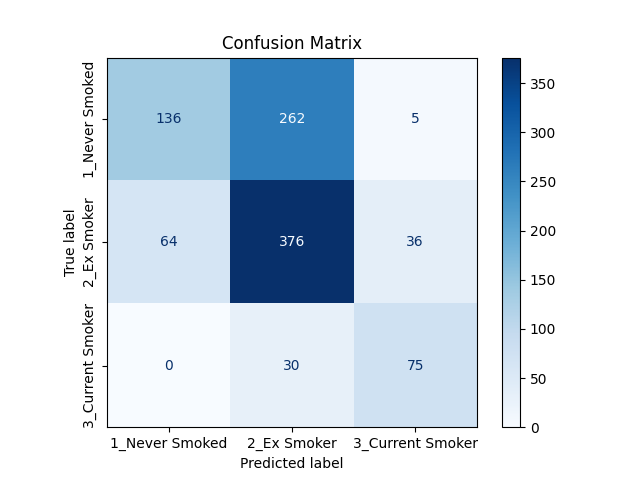
\includegraphics[width=\linewidth]{cohort2_cm.png}
        \caption{CM}
    \end{subfigure}
    \hfill
    \begin{subfigure}{0.49\textwidth}
        \centering
        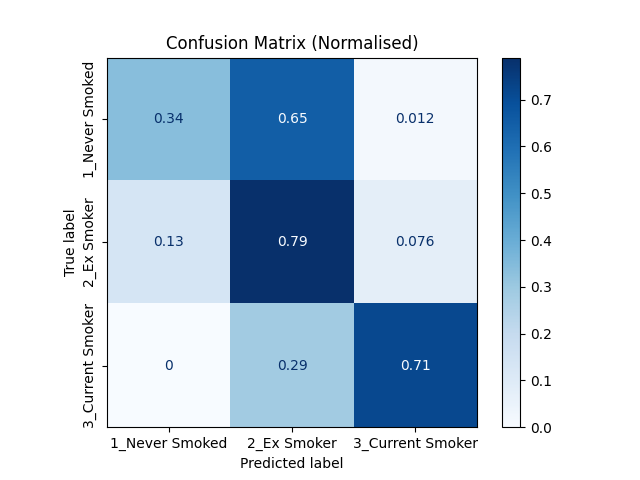
\includegraphics[width=\linewidth]{cohort2_cm_n.png}
        \caption{CM Normalised}
    \end{subfigure}
    \caption{Confusion Matrices (Cohort 2)}
\end{figure}

\begin{figure}
    \begin{subfigure}{0.48\textwidth}
        \centering
        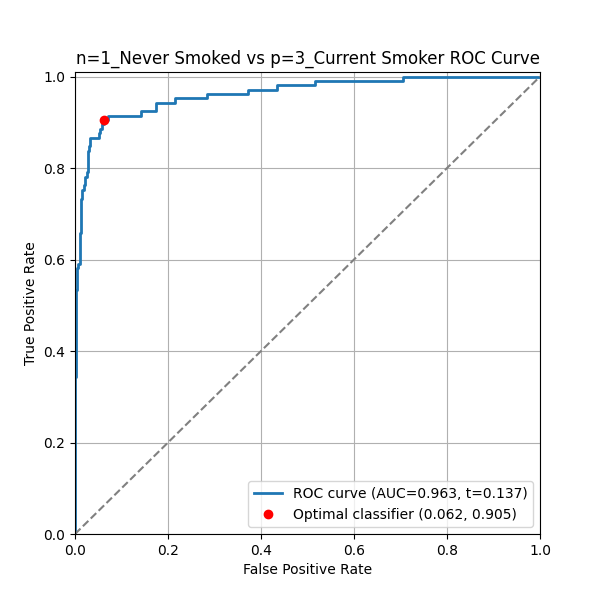
\includegraphics[width=\linewidth]{cohort2_1v3_roc.png}
        \caption{Seperation of never vs current smokers by current smoker sub-classifier}
    \end{subfigure}
    \hfill
    \begin{subfigure}{0.48\textwidth}
        \centering
        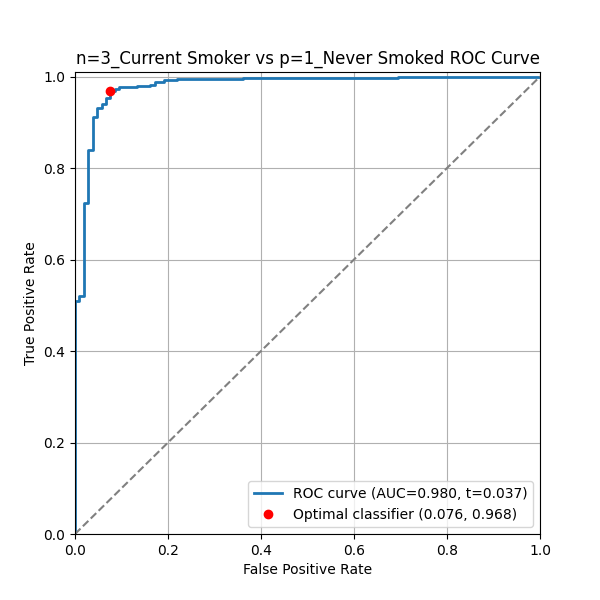
\includegraphics[width=\linewidth]{cohort2_3v1_roc.png}
        \caption{Seperation of never vs current smokers by never smoker sub-classifier}
    \end{subfigure}
    \caption{Never smoker vs current smoker sub-classifiers performance (Cohort 2)}
\end{figure}

\begin{figure}
    \begin{subfigure}{0.48\textwidth}
        \centering
        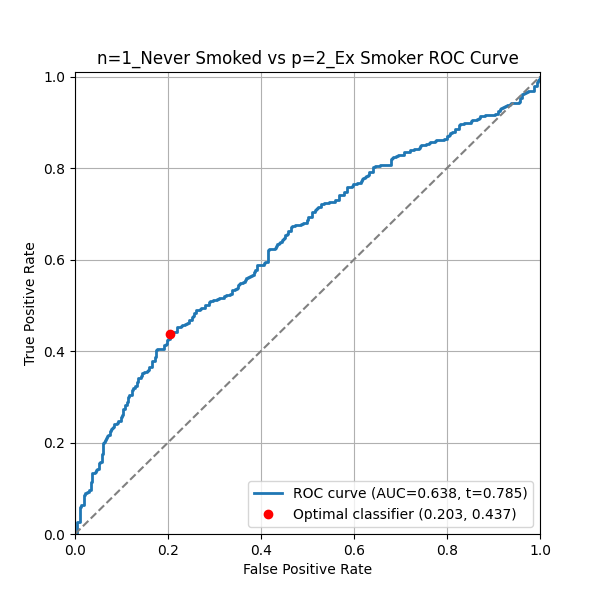
\includegraphics[width=\linewidth]{cohort2_1v2_roc.png}
        \caption{Seperation of never vs ex-smokers by ex-smoker sub-classifier}
    \end{subfigure}
    \hfill
    \begin{subfigure}{0.48\textwidth}
        \centering
        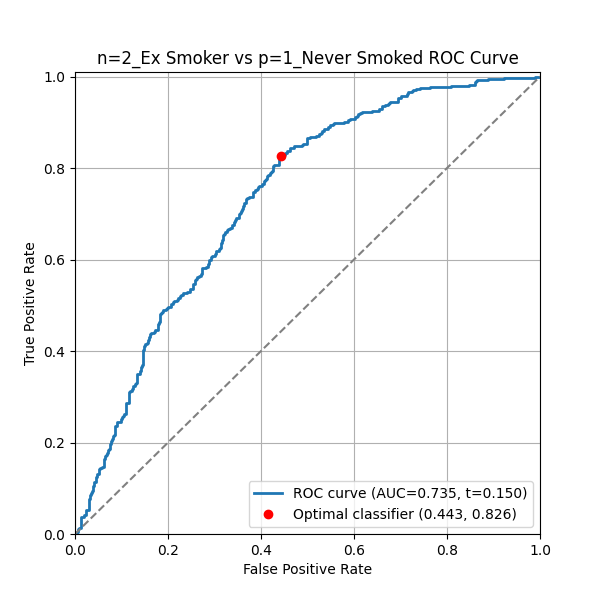
\includegraphics[width=\linewidth]{cohort2_2v1_roc.png}
        \caption{Seperation of never vs ex-smokers by never smoker sub-classifier}
    \end{subfigure}
    \caption{Never smoker vs ex-smoker sub-classifiers performance (Cohort 2)}
\end{figure}

\begin{figure}
    \begin{subfigure}{0.48\textwidth}
        \centering
        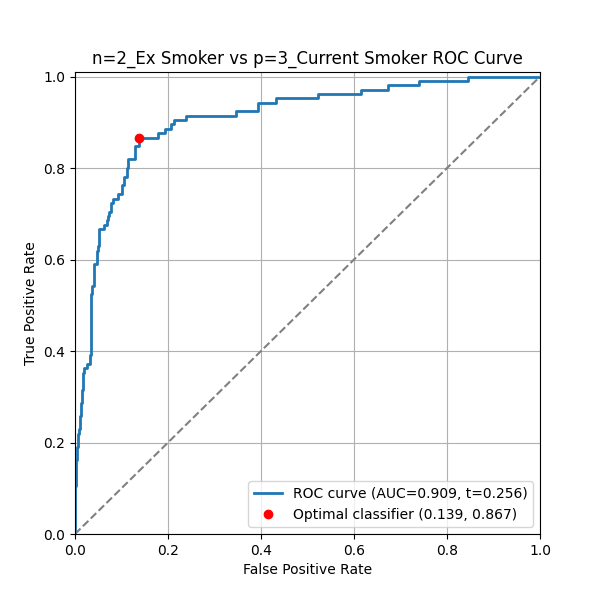
\includegraphics[width=\linewidth]{cohort2_2v3_roc.png}
        \caption{Seperation of ex vs current smokers by current smoker sub-classifier}
    \end{subfigure}
    \hfill
    \begin{subfigure}{0.48\textwidth}
        \centering
        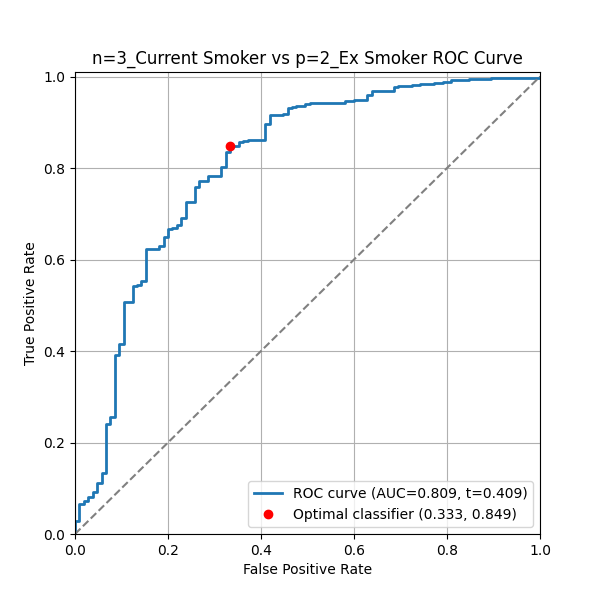
\includegraphics[width=\linewidth]{cohort2_3v2_roc.png}
        \caption{Seperation of ex vs current smokers by ex-smoker sub-classifier}
    \end{subfigure}
    \caption{Ex-smoker vs current smoker sub-classifiers performance (Cohort 2)}
\end{figure}

\begin{figure}
    \centering
    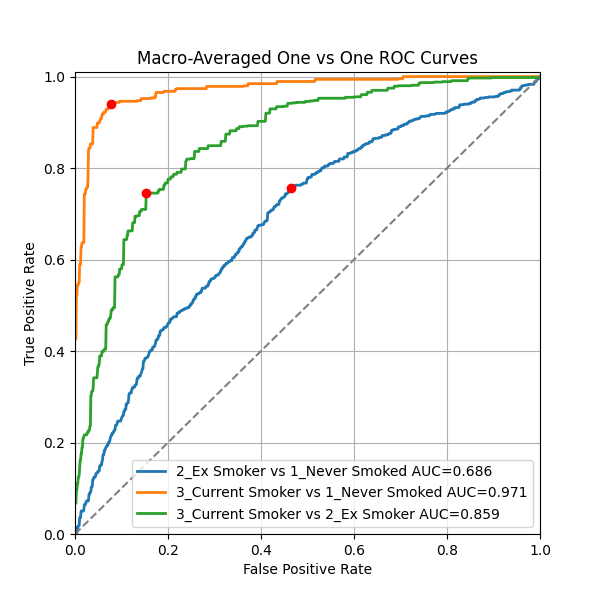
\includegraphics[width=\linewidth]{cohort2_macro_ovo_roc.png}
    \caption{Class seperation of classifier (Cohort 2)}
\end{figure}

\begin{figure}
    \centering
    \begin{subfigure}{0.48\textwidth}
        \centering
        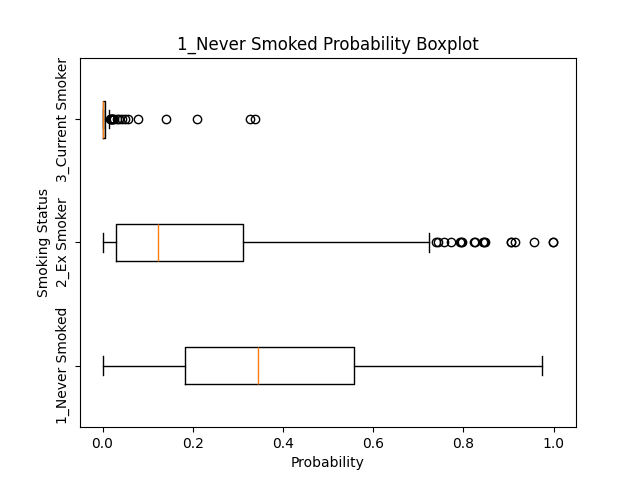
\includegraphics[width=\linewidth]{cohort2_1_boxplot.png}
        \caption{Never smoker sub-classifier probabilities across all three classes}
    \end{subfigure}
    \hfill
    \begin{subfigure}{0.48\textwidth}
        \centering
        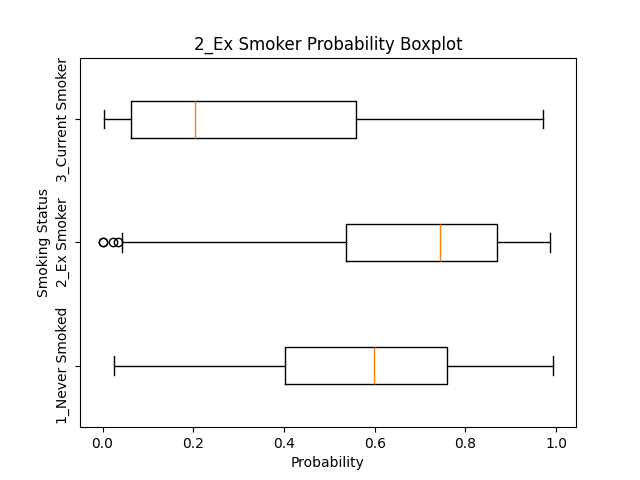
\includegraphics[width=\linewidth]{cohort2_2_boxplot.png}
        \caption{Ex-smoker sub-classifier probabilities across all three classes}
    \end{subfigure}
    \par\vspace{0.5em}
    \begin{subfigure}{0.48\textwidth}
        \centering
        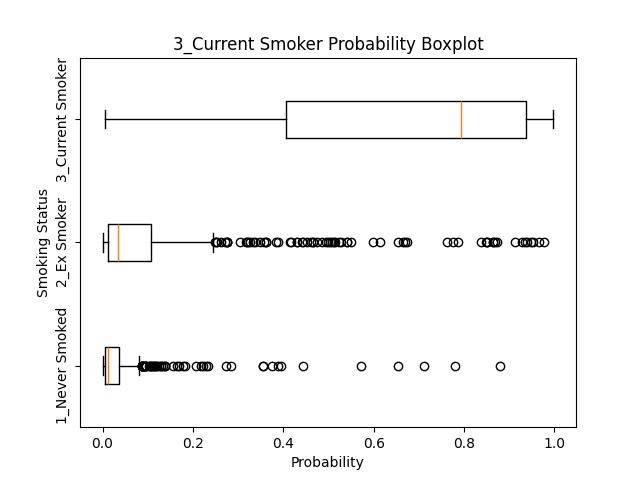
\includegraphics[width=\linewidth]{cohort2_3_boxplot.png}
        \caption{Current smoker sub-classifier probabilities across all three classes}
    \end{subfigure}
    \caption{Boxplots of probability distributions (Cohort 2)}
\end{figure}

\subsubsection{Comparison with Prior Results} \label{sec:model-comparison}

\begin{figure}
    \centering
    \begin{subfigure}{0.48\textwidth}
        \centering
        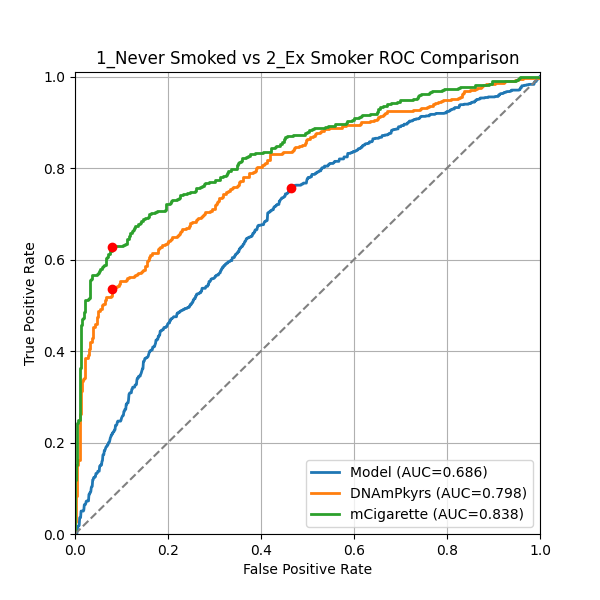
\includegraphics[width=\linewidth]{comparison_1v2_roc.png}
        \caption{comparison 1v2}
    \end{subfigure}
    \hfill
    \begin{subfigure}{0.48\textwidth}
        \centering
        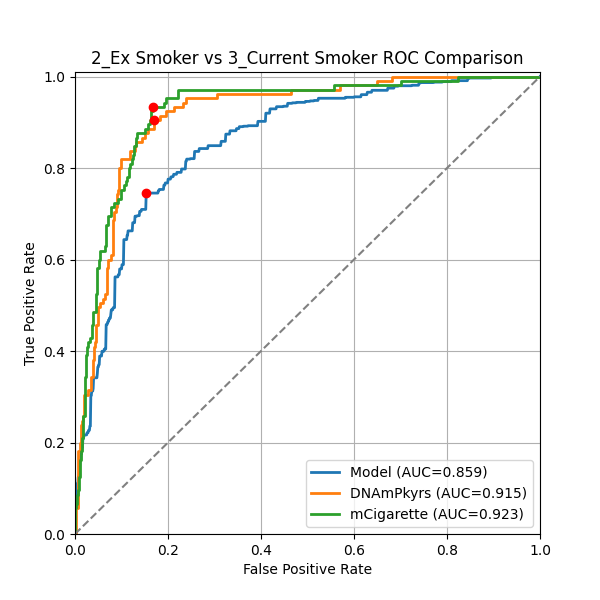
\includegraphics[width=\linewidth]{comparison_2v3_roc.png}
        \caption{comparison 2v3}
    \end{subfigure}
    \par\vspace{0.5em}
    \begin{subfigure}{0.48\textwidth}
        \centering
        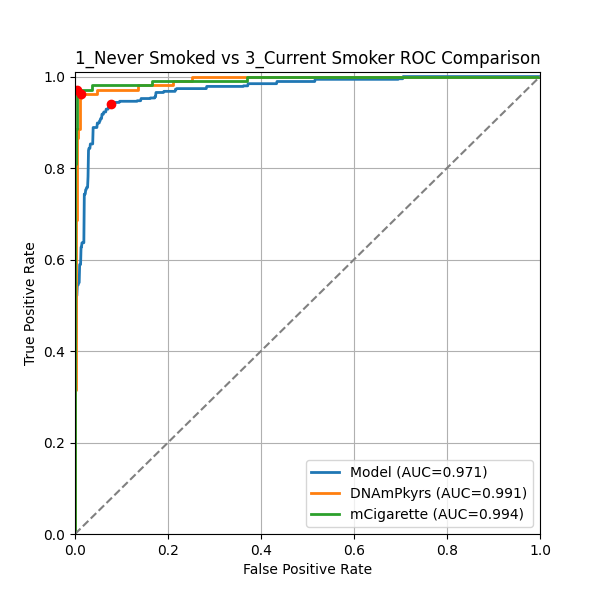
\includegraphics[width=\linewidth]{comparison_1v3_roc.png}
        \caption{comparison 1v3}
    \end{subfigure}
\end{figure}

\subsection*{Choices made in development}
\begin{itemize}
    \item class weight balancing
    \item feature pruning for cohorts, ensuring compatability
    \item direction of discovery/validation cohorts, sex being a cofounder
    \item k-fold cross validation, fold size, using stratified folds
    \item coarse-to-fine cross-validation strategy
    \item choice of scoring metric (f1-macro)
\end{itemize}

\subsection*{Comparisons to other models in validation cohort}
\begin{itemize}
    \item obviously ROC curves, etc.
    \item how many features selected during training
    \item
\end{itemize}

\subsection*{Limitations of my model vs other models}
\begin{itemize}
    \item trained only on males
    \item much smaller dataset size \((n)\)
    \item comparison of distributions of sex, age, etc in training cohorts (potential confounders)
          \begin{itemize}
              \item this is likely just a limitation of the dataset and the number of participants
          \end{itemize}
\end{itemize}

\section{Footnotes}

\subsection{Acknowledgements}

\subsection{Ethics Statement}
All participants gave written informed consent, and the study was approved by the national ethics committee. Data was anonymised and only age, biological sex and self-reported smoking values were extracted for comparison with matching whole blood DNA methylation values.

\addcontentsline{toc}{section}{References}
\printbibliography

\end{document}